\documentclass[aspectratio=169]{beamer}
\usepackage[utf8]{inputenc}
% \usepackage[italian]{babel}  % Commented out - use English instead
\usepackage{graphicx}
\usepackage{tikz}
\usepackage{listings}
\usepackage{xcolor}
\usepackage{multicol}
\usepackage{amssymb}
\usepackage{colortbl}
\usepackage{hyperref}

\usetikzlibrary{shapes,arrows,positioning,shadows,calc,shapes.geometric,mindmap,arrows.meta}

% Tema e colori
\usetheme{Madrid}
\usecolortheme{default}
\definecolor{reactblue}{RGB}{97,218,251}
\definecolor{darkblue}{RGB}{0,51,102}
\definecolor{codebg}{RGB}{245,245,245}

\setbeamercolor{structure}{fg=darkblue}
\setbeamercolor{palette primary}{bg=darkblue,fg=white}
\setbeamercolor{palette secondary}{bg=reactblue,fg=darkblue}
\setbeamercolor{title}{fg=white,bg=darkblue}
\setbeamercolor{frametitle}{fg=white,bg=darkblue}

% tcolorbox per listing avanzati
\usepackage[most]{tcolorbox}
\tcbuselibrary{listings,breakable,skins}

% Configurazione listing per codice
\lstdefinelanguage{JavaScript}{
	keywords={break, case, catch, continue, debugger, default, delete, do, else, finally, for, function, if, in, instanceof, new, return, switch, this, throw, try, typeof, var, void, while, with, const, let, class, export, import, extends, super, async, await},
	morecomment=[l]{//},
	morecomment=[s]{/*}{*/},
	morestring=[b]',
	morestring=[b]",
	sensitive=true
}

\lstset{
	basicstyle=\ttfamily\small,
	backgroundcolor=\color{codebg},
	breaklines=true,
	frame=single,
	numbers=left,
	numberstyle=\tiny\color{gray},
	keywordstyle=\color{blue},
	commentstyle=\color{green!60!black},
	stringstyle=\color{red},
	showstringspaces=false,
	escapeinside={(*@}{@*)}
}

% Informazioni del documento
\title[React.js]{React.js}
\subtitle{Tecnologie del Web}
\author{Prof. Fedeli Massimo}
\institute{IIS Fermi Sacconi Cpia}
\date{\today}

\begin{document}
	
	% ========== SLIDE 1: TITLE ==========
	\begin{frame}
		\titlepage
		\begin{center}
			
\begin{tikzpicture}[scale=0.4]
				% React logo simplified
				\draw[reactblue, ultra thick] (0,0) circle (1.5);
				\fill[reactblue] (0,0) circle (0.3);
				\draw[reactblue, ultra thick, rotate=60] (0,0) ellipse (3 and 0.8);
				\draw[reactblue, ultra thick, rotate=-60] (0,0) ellipse (3 and 0.8);
			\end{tikzpicture}
		\end{center}
	\end{frame}
	
	
	% ========== SLIDE 3: COS'È REACT ==========
	\begin{frame}{Cos'è React.js?}
		\begin{block}{Definizione}
			React.js è una \textbf{libreria JavaScript} per la creazione di interfacce utente web moderne e interattive.
		\end{block}
		
		\vspace{0.5cm}
		
		\begin{columns}
			\column{0.5\textwidth}
			\textbf{Caratteristiche principali:}
			\begin{itemize}
				\item Sviluppato da Facebook
				\item Open Source
				\item Component-based
				\item Virtual DOM
				\item Dichiarativo
			\end{itemize}
			
			\column{0.5\textwidth}
			\begin{center}
				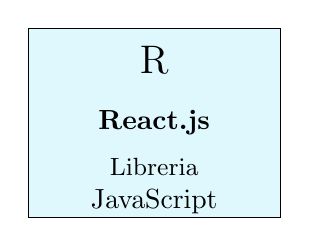
\begin{tikzpicture}[scale=0.8]
					\draw[fill=reactblue!20] (0,0) rectangle (4,3);
					\node at (2,2.5) {\Large R};
					\node at (2,1.5) {\textbf{React.js}};
					\node[align=center] at (2,0.5) {\small Libreria\\JavaScript};
				\end{tikzpicture}
			\end{center}
		\end{columns}
	\end{frame}
	
	% ========== SLIDE 4: SINGLE PAGE APPLICATION ==========
	\begin{frame}{Single Page Application (SPA)}
		\begin{columns}
			\column{0.5\textwidth}
			\textbf{Approccio Tradizionale:}
			\begin{center}
				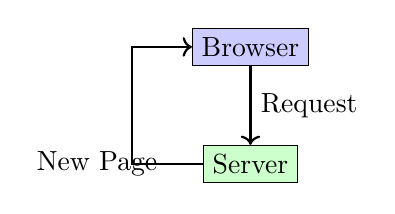
\begin{tikzpicture}[scale=0.6, node distance=1cm]
					\node[draw, rectangle, fill=blue!20] (browser1) {Browser};
					\node[draw, rectangle, fill=green!20, below=of browser1] (server1) {Server};
					\draw[->, thick] (browser1) -- node[right] {Request} (server1);
					\draw[->, thick] (server1.west) -- node[left] {New Page} ++(-1.5,0) |- (browser1.west);
				\end{tikzpicture}
			\end{center}
			\small Caricamento di nuove pagine ad ogni interazione
			
			\column{0.5\textwidth}
			\textbf{Single Page Application:}
			\begin{center}
				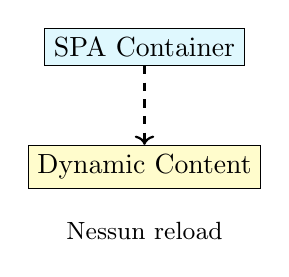
\begin{tikzpicture}[scale=0.6, node distance=1cm]
					\node[draw, rectangle, fill=reactblue!20] (spa) {SPA Container};
					\node[draw, rectangle, fill=yellow!20, below=of spa] (content) {Dynamic Content};
					\draw[->, thick, dashed] (spa) -- (content);
					\node[below=0.3cm of content] {\small Nessun reload};
				\end{tikzpicture}
			\end{center}
			\small La pagina evolve dinamicamente senza ricaricare
		\end{columns}
	\end{frame}
	
	
	% ========== SLIDE 5: VIRTUAL DOM ==========
	\begin{frame}{Virtual DOM}
		\begin{center}
			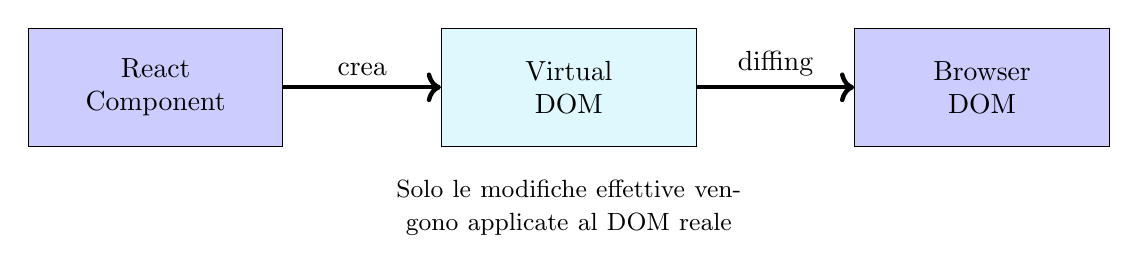
\begin{tikzpicture}[
				node distance=2cm,
				box/.style={rectangle, draw, fill=blue!20, text width=3cm, align=center, minimum height=1.5cm},
				vbox/.style={rectangle, draw, fill=reactblue!20, text width=3cm, align=center, minimum height=1.5cm}
				]
				\node[box] (react) {React\\Component};
				\node[vbox, right=of react] (vdom) {Virtual\\DOM};
				\node[box, right=of vdom] (dom) {Browser\\DOM};
				
				\draw[->, ultra thick] (react) -- node[above] {crea} (vdom);
				\draw[->, ultra thick] (vdom) -- node[above] {diffing} (dom);
				
				\node[below=0.3cm of vdom, text width=6cm, align=center] {
					\small Solo le modifiche effettive vengono applicate al DOM reale
				};
			\end{tikzpicture}
		\end{center}
		
		\vspace{0.5cm}
		
		\begin{block}{Vantaggi del Virtual DOM}
			\begin{itemize}
				\item \textbf{Performance}: aggiornamenti ottimizzati
				\item \textbf{Efficienza}: solo i cambiamenti reali vengono applicati
				\item \textbf{Astrazione}: lo sviluppatore non manipola direttamente il DOM
			\end{itemize}
		\end{block}
	\end{frame}
	
	
	\begin{frame}
		\frametitle{Il Virtual DOM di React}
		
		\begin{block}{Definizione}
			Il \textbf{Virtual DOM} è una rappresentazione in memoria (in JavaScript) della struttura DOM reale della pagina.
		\end{block}
		
		\vspace{0.5cm}
		
		\begin{itemize}
			\item È una copia leggera dell'albero DOM effettivo del browser
			\item Mantenuto da React come oggetto JavaScript
			\item Permette operazioni veloci senza toccare il DOM reale
		\end{itemize}
		
	\end{frame}
	
	% Slide 2: Come funziona
	\begin{frame}
		\frametitle{Come Funziona il Virtual DOM}
		
		\textbf{Processo di aggiornamento:}
		
		\begin{enumerate}
			\item \textbf{Creazione del nuovo Virtual DOM}\\
			React crea un nuovo albero Virtual DOM con i nuovi dati
			
			\vspace{0.3cm}
			
			\item \textbf{Confronto (Diffing)}\\
			Algoritmo efficiente confronta il nuovo Virtual DOM con la versione precedente
			
			\vspace{0.3cm}
			
			\item \textbf{Riconciliazione}\\
			React calcola il modo più efficiente per aggiornare il DOM reale
			
			\vspace{0.3cm}
			
			\item \textbf{Aggiornamento del DOM reale}\\
			Solo le parti effettivamente cambiate vengono aggiornate nel browser
		\end{enumerate}
		
	\end{frame}
	
	% Slide 3: Vantaggi
	\begin{frame}
		\frametitle{Vantaggi del Virtual DOM}
		
		\begin{block}{Perché è efficiente?}
			Manipolare direttamente il DOM è costoso in termini di performance
		\end{block}
		
		\vspace{0.5cm}
		
		\textbf{Vantaggi principali:}
		
		\begin{itemize}
			\item[$\checkmark$] Le operazioni sul Virtual DOM sono molto più veloci (solo JavaScript in memoria)
			
			\vspace{0.2cm}
			
			\item[$\checkmark$] React raggruppa molteplici cambiamenti e li applica in un'unica operazione
			
			\vspace{0.2cm}
			
			\item[$\checkmark$] Vengono aggiornati solo gli elementi effettivamente modificati
			
			\vspace{0.2cm}
			
			\item[$\checkmark$] Ideale per applicazioni con interfacce dinamiche che cambiano frequentemente
		\end{itemize}
		
	\end{frame}
	
	% ========== SLIDE 6: SETUP AMBIENTE ==========
	\begin{frame}[fragile]{Preparazione Ambiente di Sviluppo}
		\begin{block}{In Laboratorio}
			\begin{enumerate}
				\item Accedere a \texttt{C:\textbackslash Applicativi\textbackslash TecnologieWeb\textbackslash}
				\item Copiare \texttt{react.zip} su pen drive USB
				\item Scompattare il file (operazione lunga)
				\item Risultato: directory \texttt{my-app} pronta
			\end{enumerate}
		\end{block}
		
		\begin{block}{Da Casa}
			\begin{lstlisting}[language=bash]
				# 1. Installare Node.js da https://nodejs.org
				# 2. Creare applicazione React
				npx create-react-app my-app
				# 3. Avviare l'applicazione
				cd my-app
				npm start
			\end{lstlisting}
		\end{block}
	\end{frame}
	
	% ========== SLIDE 7: STRUTTURA PROGETTO ==========
	\begin{frame}{Struttura del Progetto React}
		\begin{columns}
			\column{0.5\textwidth}
			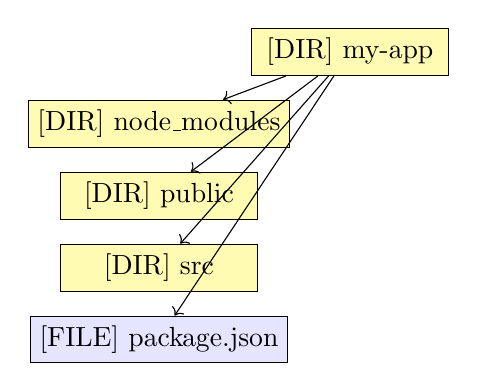
\begin{tikzpicture}[
				folder/.style={draw, rectangle, fill=yellow!30, minimum width=2.5cm, minimum height=0.6cm},
				file/.style={draw, rectangle, fill=blue!10, minimum width=2.5cm, minimum height=0.5cm}
				]
				\node[folder] (root) at (0,0) {[DIR]\ my-app};
				\node[folder, below left=0.3cm and -0.5cm of root] (node) {[DIR]\ node\_modules};
				\node[folder, below=0.3cm of node] (public) {[DIR]\ public};
				\node[folder, below=0.3cm of public] (src) {[DIR]\ src};
				\node[file, below=0.3cm of src] (package) {[FILE]\ package.json};
				
				\draw[->] (root) -- (node);
				\draw[->] (root) -- (public);
				\draw[->] (root) -- (src);
				\draw[->] (root) -- (package);
			\end{tikzpicture}
			
			\column{0.5\textwidth}
			\textbf{Descrizione cartelle:}
			\begin{itemize}
				\item \texttt{node\_modules}: librerie e dipendenze
				\item \texttt{public}: template HTML
				\item \texttt{src}: codice sorgente JavaScript
				\item \texttt{package.json}: configurazione progetto
			\end{itemize}
		\end{columns}
		
		\vspace{0.5cm}
		\begin{alertblock}{Comando di avvio}
			\texttt{npm start} $\rightarrow$ Avvia server su porta 3000
		\end{alertblock}
	\end{frame}
	
	
	\begin{frame}[fragile]
		\frametitle{Struttura di un Progetto React}
		
		\begin{block}{Cartelle e File Principali}
			\small
			\texttt{my-react-app/}
			\begin{itemize}
				\item \texttt{node\_modules/} - Librerie e dipendenze installate
				\item \texttt{public/} - File statici accessibili pubblicamente
				\begin{itemize}
					\item \texttt{index.html} - Template HTML principale
					\item \texttt{favicon.ico} - Icona del sito
				\end{itemize}
				\item \texttt{src/} - Codice sorgente dell'applicazione
				\begin{itemize}
					\item \texttt{index.js} - Punto di ingresso dell'app
					\item \texttt{App.js} - Componente principale
					\item \texttt{App.css} - Stili del componente principale
					\item \texttt{components/} - Componenti riutilizzabili
				\end{itemize}
				\item \texttt{package.json} - Configurazione e dipendenze del progetto
				\item \texttt{.gitignore} - File da ignorare in Git
			\end{itemize}
		\end{block}
		
	\end{frame}
	% ========== SLIDE 8: JSX ==========

		\begin{frame}[fragile]{JSX in React}
		\begin{block}{Cos'è JSX}
			JSX è un'estensione sintattica di JavaScript che permette di descrivere l'interfaccia utente
			utilizzando una sintassi simile all'HTML.  
			Viene compilato in chiamate a \texttt{React.createElement}.
		\end{block}
		\begin{itemize}
			\item JSX non è obbligatorio, ma rende il codice più leggibile.
			\item Il browser non lo interpreta direttamente: serve una fase di trasformazione (Babel).
			\item Permette di combinare logica JavaScript e struttura dell'interfaccia.
		\end{itemize}
	\end{frame}
	
	
	\begin{frame}[fragile]{JSX - JavaScript XML}
		\begin{block}{Cos'è JSX?}
			Sintassi che permette di scrivere tag HTML all'interno di codice JavaScript
		\end{block}
		
		\begin{columns}
			\column{0.5\textwidth}
			\textbf{Senza JSX:}
			\begin{tcblisting}{listing engine=listings, breakable, left=2mm, right=2mm, top=1mm, bottom=1mm}
				const element = 
				React.createElement('h1',
				{classNam6e: 'greeting'},
				'Hello, World!'
				);
			\end{tcblisting}
			\column{0.5\textwidth}
			\textbf{Con JSX:}
			\begin{tcblisting}{listing engine=listings, breakable, left=2mm, right=2mm, top=1mm, bottom=1mm}
				const element = (<h1 
				className="greeting">
				Hello, World! </h1>
				);
			\end{tcblisting}
		\end{columns}
	
	\end{frame}
	
	\begin{frame}
	\begin{center}
	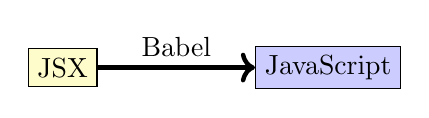
\begin{tikzpicture}
		\node[draw, rectangle, fill=yellow!20] (jsx) {JSX};
		\node[draw, rectangle, fill=blue!20, right=2cm of jsx] (js) {JavaScript};
		\draw[->, ultra thick] (jsx) -- node[above] {Babel} (js);
	\end{tikzpicture}
\end{center}
	\end{frame}
	
	

	
	
	% ========== SLIDE 9: COMPONENTI INTRO ==========
	\begin{frame}{Approccio a Componenti}
		\begin{center}
			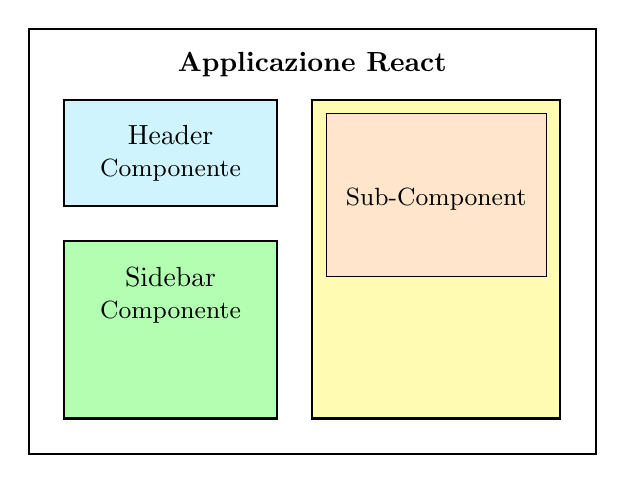
\begin{tikzpicture}[scale=0.9]
				% Interfaccia principale
				\draw[thick] (0,0) rectangle (8,6);
				\node at (4,5.5) {\textbf{Applicazione React}};
				
				% Componenti
				\draw[fill=reactblue!30, thick] (0.5,3.5) rectangle (3.5,5);
				\node at (2,4.5) {Header};
				\node at (2,4) {\small Componente};
				
				\draw[fill=green!30, thick] (0.5,0.5) rectangle (3.5,3);
				\node at (2,2.5) {Sidebar};
				\node at (2,2) {\small Componente};
				
				\draw[fill=yellow!30, thick] (4,0.5) rectangle (7.5,5);
				\node at (5.75,4.5) {Main Content};
				\node at (5.75,4) {\small Componente};
				
				% Sotto-componenti
				\draw[fill=orange!20] (4.2,2.5) rectangle (7.3,4.8);
				\node[font=\small] at (5.75,3.6) {Sub-Component};
			\end{tikzpicture}
		\end{center}
	\end{frame}
\begin{frame}[fragile]
	\frametitle{Vantaggi dei Componenti React}
	
	\begin{block}{Riusabilità}
		\textbf{Componenti utilizzabili ovunque nell'applicazione}
		\begin{itemize}
			\item Scrivi una volta, usa molte volte
			\item Risparmio di tempo e codice duplicato
			\item Coerenza visiva e funzionale in tutta l'app
		\end{itemize}
	\end{block}
	
	\vspace{0.3cm}
	
	\textbf{Esempio:}
	\begin{lstlisting}[basicstyle=\ttfamily\tiny]
		// Definisci il componente una volta
		function Button({ testo, onClick }) {
			return <button onClick={onClick}>{testo}</button>;
		}
		
		// Riutilizzalo ovunque
		<Button testo="Salva" onClick={handleSave} />
		<Button testo="Elimina" onClick={handleDelete} />
		<Button testo="Annulla" onClick={handleCancel} />
	\end{lstlisting}
	
\end{frame}

\begin{frame}[fragile]
	\frametitle{Vantaggi dei Componenti React (continua)}
	
	\begin{block}{Modularità}
		\textbf{Costruzione dell'interfaccia per composizione}
		\begin{itemize}
			\item Suddivisione in unità piccole e gestibili
			\item Ogni componente ha una responsabilità specifica
			\item Facile combinare componenti per creare UI complesse
			\item Sviluppo parallelo e isolato
		\end{itemize}
	\end{block}
	
	\vspace{0.3cm}
	
	\textbf{Esempio di composizione:}
	\begin{lstlisting}[basicstyle=\ttfamily\tiny]
		function App() {
			return (
			<div>
			<Header />
			<Sidebar />
			<MainContent>
			<ArticleList />
			<Pagination />
			</MainContent>
			<Footer />
			</div>
			);
		}
	\end{lstlisting}
	
\end{frame}

\begin{frame}[fragile]
	\frametitle{Vantaggi dei Componenti React (continua)}
	
	\begin{block}{Manutenibilità}
		\textbf{Focus separato su logica e layout}
		\begin{itemize}
			\item Codice organizzato e facilmente comprensibile
			\item Bug più facili da individuare e correggere
			\item Testing semplificato (componenti isolati)
			\item Aggiornamenti localizzati senza effetti collaterali
			\item Documentazione più chiara
		\end{itemize}
	\end{block}
	
	\vspace{0.3cm}	
\end{frame}

\begin{frame}[fragile]
	\frametitle{Esempio: Componente Manutenibile}
	
	\begin{lstlisting}
		// Modifica solo il componente necessario
		function UserCard({ user }) {
			// Logica isolata
			const formattedDate = formatDate(user.registrationDate);
			
			// Layout chiaro
			return (
			<div className="card">
			<img src={user.avatar} alt={user.name} />
			<h3>{user.name}</h3>
			<p>Iscritto dal: {formattedDate}</p>
			</div>
			);
		}
	\end{lstlisting}
	
\end{frame}

\begin{frame}
\begin{block}{Vantaggi di questo approccio}
	\begin{itemize}
		\item Logica separata dalla presentazione
		\item Facile da testare e modificare
		\item Codice chiaro e leggibile
	\end{itemize}
\end{block}

\end{frame}

\begin{frame}
	\frametitle{Riepilogo Vantaggi}
	
	\begin{center}
		\begin{tabular}{|l|p{8cm}|}
			\hline
			\textbf{Vantaggio} & \textbf{Beneficio Pratico} \\
			\hline
			\textbf{Riusabilità} & Riduzione del codice duplicato e tempi di sviluppo più brevi \\
			\hline
			\textbf{Modularità} & Architettura scalabile e sviluppo team più efficiente \\
			\hline
			\textbf{Manutenibilità} & Debug più rapido e aggiornamenti sicuri \\
			\hline
		\end{tabular}
	\end{center}
	
	\vspace{0.5cm}
	
	\begin{alertblock}{Best Practice}
		Mantieni i componenti piccoli, focalizzati e con responsabilità singole (Single Responsibility Principle)
	\end{alertblock}
	
\end{frame}
	
	% ========== SLIDE 10: TIPI DI COMPONENTI ==========
	\begin{frame}{Tipi di Componenti}
		\begin{columns}
			\column{0.5\textwidth}
			\begin{block}{Function Component}
				\begin{center}
					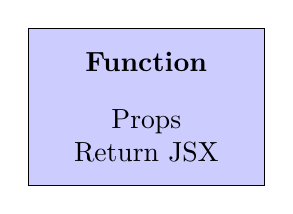
\begin{tikzpicture}
						\node[draw, rectangle, fill=blue!20, minimum width=3cm, minimum height=2cm, align=center] {
							\textbf{Function}\\[0.3cm]
							Props \\
							Return JSX
						};
					\end{tikzpicture}
				\end{center}
				\begin{itemize}
					\item Più semplici
					\item Stateless
					\item Solo props
				\end{itemize}
			\end{block}
			
			\column{0.5\textwidth}
			\begin{block}{Class Component}
				\begin{center}
					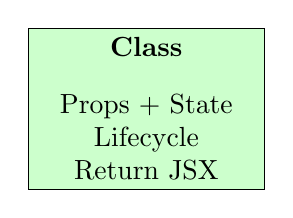
\begin{tikzpicture}
						\node[draw, rectangle, fill=green!20, minimum width=3cm, minimum height=2cm, align=center] {
							\textbf{Class}\\[0.3cm]
							Props + State\\
							Lifecycle\\
							Return JSX
						};
					\end{tikzpicture}
				\end{center}
				\begin{itemize}
					\item Più complessi
					\item Stateful
					\item Props + State
				\end{itemize}
			\end{block}
		\end{columns}
		
		\vspace{0.5cm}
		\begin{alertblock}{Nota}
			Entrambi i tipi devono restituire JSX tramite \texttt{return}
		\end{alertblock}
	\end{frame}
	
	
	\begin{frame}[fragile]
		\frametitle{Cosa sono i Componenti React?}
		
		\begin{block}{Definizione}
			I componenti sono i \textbf{mattoni fondamentali} di un'applicazione React. Ogni componente è una funzione o classe JavaScript che accetta input (props) e restituisce elementi React che descrivono l'interfaccia utente.
		\end{block}
		
		\vspace{0.5cm}
		
		\begin{columns}[T]
			\column{0.48\textwidth}
			\textbf{Caratteristiche:}
			\begin{itemize}
				\item Indipendenti e riutilizzabili
				\item Accettano input (props)
				\item Restituiscono JSX
				\item Possono avere stato interno
			\end{itemize}
			
			\column{0.48\textwidth}
			\textbf{Analogia:}
			\begin{alertblock}{Componenti = Funzioni}
				Come le funzioni in matematica, i componenti trasformano input in output
			\end{alertblock}
		\end{columns}
		
	\end{frame}
	
	\begin{frame}[fragile]
		\frametitle{Tipi di Componenti}
		
		\begin{columns}
			\column{0.5\textwidth}
			\begin{block}{Function Component}
				\begin{center}
					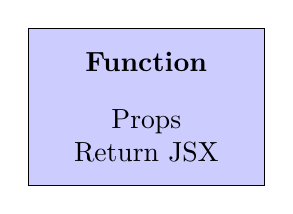
\begin{tikzpicture}
						\node[draw, rectangle, fill=blue!20, minimum width=3cm, minimum height=2cm, align=center] {
							\textbf{Function}\\[0.3cm]
							Props \\
							Return JSX
						};
					\end{tikzpicture}
				\end{center}
				\begin{itemize}
					\item Più semplici
					\item Moderni (con Hooks)
					\item Raccomandati oggi
				\end{itemize}
			\end{block}
			
			\column{0.5\textwidth}
			\begin{block}{Class Component}
				\begin{center}
					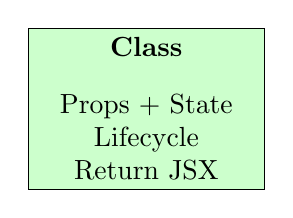
\begin{tikzpicture}
						\node[draw, rectangle, fill=green!20, minimum width=3cm, minimum height=2cm, align=center] {
							\textbf{Class}\\[0.3cm]
							Props + State\\
							Lifecycle\\
							Return JSX
						};
					\end{tikzpicture}
				\end{center}
				\begin{itemize}
					\item Più complessi
					\item Approccio tradizionale
					\item Meno usati oggi
				\end{itemize}
			\end{block}
		\end{columns}
		
	\end{frame}
	
	\begin{frame}[fragile]
		\frametitle{Function Component - Esempio}
		
		\textbf{Componente semplice:}
		\begin{lstlisting}
			function Benvenuto(props) {
				return <h1>Ciao, {props.nome}!</h1>;
			}
			
			// Utilizzo
			<Benvenuto nome="Mario" />
		\end{lstlisting}
		
		\vspace{0.3cm}
		
		\textbf{Con destructuring (più comune):}
		\begin{lstlisting}
			function Benvenuto({ nome }) {
				return <h1>Ciao, {nome}!</h1>;
			}
		\end{lstlisting}
		
		\vspace{0.3cm}
		
		\textbf{Arrow function (sintassi moderna):}
		\begin{lstlisting}
			const Benvenuto = ({ nome }) => {
				return <h1>Ciao, {nome}!</h1>;
			};
		\end{lstlisting}
		
	\end{frame}
	
	\begin{frame}[fragile]
		\frametitle{Function Component con Hooks}
		
		\textbf{Componente con stato (useState):}
		\begin{lstlisting}
			import { useState } from 'react';
			
			function Contatore() {
				const [count, setCount] = useState(0);
				
				return (
				<div>
				<p>Hai cliccato {count} volte</p>
				<button onClick={() => setCount(count + 1)}>
				Incrementa
				</button>
				</div>
				);
			}
		\end{lstlisting}
		
		\vspace{0.3cm}
		
		\begin{block}{Hooks}
			Gli Hooks permettono ai function component di avere stato e altre funzionalità che prima erano disponibili solo nei class component.
		\end{block}
		
	\end{frame}
	
	\begin{frame}[fragile]
		\frametitle{Class Component - Esempio}
		
		\begin{lstlisting}
			import React, { Component } from 'react';
			
			class Contatore extends Component {
				constructor(props) {
					super(props);
					this.state = { count: 0 };
				}
				
				incrementa = () => {
					this.setState({ count: this.state.count + 1 });
				}
				
				render() {
					return (
					<div>
					<p>Hai cliccato {this.state.count} volte</p>
					<button onClick={this.incrementa}>
					Incrementa
					</button>
					</div>
					);
				}
			}
		\end{lstlisting}
		
	\end{frame}
	
	\begin{frame}
		\frametitle{Confronto: Function vs Class Component}
		
		\begin{center}
			\begin{tabular}{|l|p{3.5cm}|p{3.5cm}|}
				\hline
				\textbf{Aspetto} & \textbf{Function Component} & \textbf{Class Component} \\
				\hline
				Sintassi & Più semplice & Più verbosa \\
				\hline
				Stato & Hooks (useState) & this.state \\
				\hline
				Props & Parametro funzione & this.props \\
				\hline
				Lifecycle & useEffect & componentDidMount, ecc. \\
				\hline
				Performance & Leggermente migliori & Buone \\
				\hline
				Trend & \textcolor{green}{\textbf{Raccomandati}} & Legacy \\
				\hline
			\end{tabular}
		\end{center}
		
		\vspace{0.5cm}
		
		\begin{alertblock}{Best Practice Attuale}
			React raccomanda l'uso di \textbf{Function Component con Hooks} per tutti i nuovi progetti.
		\end{alertblock}
		
	\end{frame}
	
	\begin{frame}[fragile]
		\frametitle{Anatomia di un Componente}
		
		\begin{lstlisting}
			// 1. Import necessari
			import React, { useState } from 'react';
			
			// 2. Definizione del componente
			function MioComponente({ titolo, descrizione }) {
				// 3. Stato locale (opzionale)
				const [attivo, setAttivo] = useState(false);
				
				// 4. Funzioni helper (opzionale)
				const handleClick = () => {
					setAttivo(!attivo);
				};
				
				// 5. Return del JSX
				return (
				<div className={attivo ? 'active' : ''}>
				<h2>{titolo}</h2>
				<p>{descrizione}</p>
				<button onClick={handleClick}>Toggle</button>
				</div>
				);
			}
			
			// 6. Export del componente
			export default MioComponente;
		\end{lstlisting}
		
	\end{frame}
	
	\begin{frame}
		\frametitle{Props: Comunicazione tra Componenti}
		
		\begin{block}{Cosa sono le Props?}
			Le \textbf{props} (properties) sono gli argomenti passati ai componenti React. Funzionano come i parametri delle funzioni JavaScript.
		\end{block}
		
		\vspace{0.3cm}
		
		\textbf{Caratteristiche delle props:}
		\begin{itemize}
			\item \textbf{Read-only}: non possono essere modificate dal componente
			\item \textbf{Unidirezionali}: fluiscono dal genitore al figlio
			\item \textbf{Qualsiasi tipo}: stringhe, numeri, oggetti, funzioni, componenti
			\item \textbf{Dinamiche}: possono cambiare nel tempo
		\end{itemize}
		
		\vspace{0.3cm}
		
		\begin{alertblock}{Regola d'oro}
			Un componente non deve mai modificare le proprie props. Deve comportarsi come una funzione pura rispetto ai suoi input.
		\end{alertblock}
		
	\end{frame}
	
	\begin{frame}[fragile]
		\frametitle{Esempio Completo: Card Component}
		
		\begin{lstlisting}
			function UserCard({ nome, email, avatar, isOnline }) {
				return (
				<div className="user-card">
				<img src={avatar} alt={nome} />
				<div className="user-info">
				<h3>{nome}</h3>
				<p>{email}</p>
				{isOnline && <span className="badge">Online</span>}
				</div>
				</div>
				);
			}
			
			// Utilizzo
			function App() {
				return (
				<div>
				<UserCard 
				nome="Mario Rossi"
				email="mario@example.com"
				avatar="/img/mario.jpg"
				isOnline={true}
				/>
				</div>
				);
			}
		\end{lstlisting}
		
	\end{frame}
	
	\begin{frame}
		\frametitle{Riepilogo Componenti}
		
		\begin{block}{Punti Chiave}
			\begin{enumerate}
				\item I componenti sono i \textbf{blocchi costruttivi} di React
				\item Possono essere \textbf{Function} o \textbf{Class} (usa Function!)
				\item Accettano \textbf{props} come input
				\item Restituiscono \textbf{JSX} come output
				\item Possono avere \textbf{stato interno} (con Hooks)
				\item Sono \textbf{componibili} e \textbf{riutilizzabili}
			\end{enumerate}
		\end{block}
		
		\vspace{0.5cm}
		
		\begin{center}
			\Large{\textbf{Componente = Input (Props) + Logica + Output (JSX)}}
		\end{center}
		
	\end{frame}
	
	
	% ========== SLIDE 11: FUNCTION COMPONENT ==========
\begin{frame}[fragile]{Function Component --- Esempio}
	\begin{lstlisting}[language=JavaScript]
		function Welcome(props) {
			return <h1>Benvenuto, {props.name}!</h1>;
		}
		
		// Utilizzo
		<Welcome name="Massimo" />
	\end{lstlisting}
	
	\vspace{0.4cm}
	
	\begin{center}
		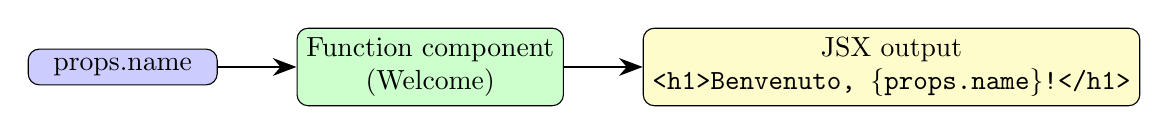
\begin{tikzpicture}[node distance=1cm,
			box/.style={draw, rectangle, rounded corners, minimum width=2.4cm, align=center},
			arrow/.style={-{Stealth[length=3mm]}, thick}]
			\node[box, fill=blue!20] (props) {props.name};
			\node[box, fill=green!20, right=of props] (func) {Function component\\(Welcome)};
			\node[box, fill=yellow!20, right=of func] (jsx) {JSX output\\\texttt{<h1>Benvenuto, \{props.name\}!</h1>}};
			
			\draw[arrow] (props) -- (func);
			\draw[arrow] (func) -- (jsx);
		\end{tikzpicture}
	\end{center}
	
	\begin{block}{Caratteristiche}
		\begin{itemize}
			\item Componenti definite come funzioni: accettano \texttt{props} e restituiscono JSX.
			\item Il nome del componente deve iniziare con lettera maiuscola (convenzione di React).
			\item Ideali per componenti di presentazione; facilmente combinabili con Hooks.
		\end{itemize}
	\end{block}
\end{frame}

	
	% ========== SLIDE 12: CLASS COMPONENT ==========
	\begin{frame}[fragile]{Class Component - Esempio}
		\begin{lstlisting}[language=JavaScript, basicstyle=\ttfamily\footnotesize]
			class Welcome extends React.Component {
				render() {
					return <h1>Benvenuto, {this.props.name}!</h1>;
				}
			}
			
			// Utilizzo
			<Welcome name="Massimo" />
		\end{lstlisting}
		
		\begin{block}{Accesso alle props}
			Nelle classi si usa \texttt{this.props} invece di \texttt{props}
		\end{block}
		
		\begin{center}
			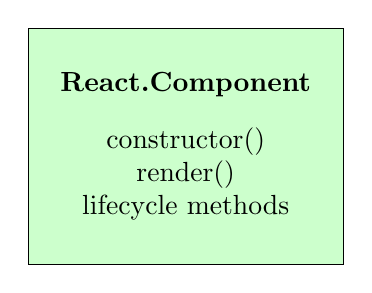
\begin{tikzpicture}[scale=0.8]
				\node[draw, rectangle, fill=green!20, minimum width=4cm, minimum height=3cm, align=center] {
					\textbf{React.Component}\\[0.3cm]
					constructor()\\
					render()\\
					lifecycle methods
				};
			\end{tikzpicture}
		\end{center}
	\end{frame}
	
	% ========== SLIDE 13: PROPS ==========
	\begin{frame}{Props - Proprietà Immutabili}
		\begin{center}
			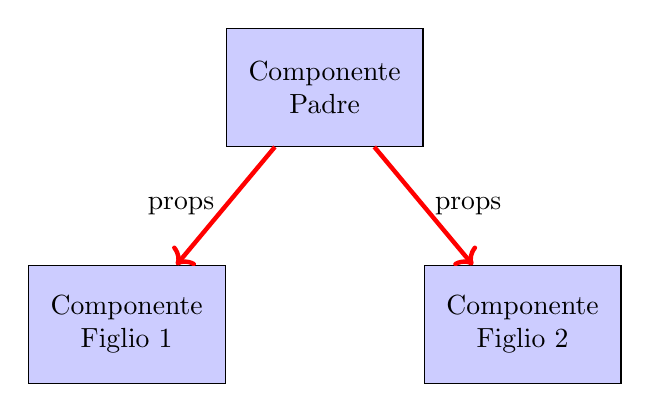
\begin{tikzpicture}[
				node distance=2cm,
				component/.style={rectangle, draw, fill=blue!20, minimum width=2.5cm, minimum height=1.5cm, align=center}
				]
				\node[component] (parent) {Componente\\Padre};
				\node[component, below left=1.5cm and 0cm of parent] (child1) {Componente\\Figlio 1};
				\node[component, below right=1.5cm and 0cm of parent] (child2) {Componente\\Figlio 2};
				
				\draw[->, ultra thick, red] (parent) -- node[left, black] {props} (child1);
				\draw[->, ultra thick, red] (parent) -- node[right, black] {props} (child2);
			\end{tikzpicture}
		\end{center}
		
		\begin{block}{Caratteristiche delle Props}
			\begin{itemize}
				\item \textbf{Immutabili}: non possono essere modificate dal componente figlio
				\item \textbf{Unidirezionali}: flusso dati dal padre al figlio
				\item \textbf{Configurazione}: usate per parametrizzare i componenti
			\end{itemize}
		\end{block}
	\end{frame}
	
	% ========== SLIDE 14: STATE ==========
	% Richiede nel preambolo:
	% \usepackage{tikz}
	% \usetikzlibrary{positioning,arrows.meta}
	\begin{frame}[fragile]{State — Stato del componente}
		\begin{columns}[T]
			\begin{column}{0.50\textwidth}
				\begin{lstlisting}[language=JavaScript,basicstyle=\ttfamily\small]
					class Counter extends React.Component {
						constructor(props) {
							super(props);
							this.state = { count: 0 };
							this.increment = this.increment.bind(this);
						}
						
						increment() {
							this.setState((prevState) => ({ count: prevState.count + 1 }));
						}
						
						render() {
							return (
							<div>
							<p>{this.state.count}</p>
							<button onClick={this.increment}>Aggiungi</button>
							</div>
							);
						}
					}
				\end{lstlisting}
			\end{column}
			
			\begin{column}{0.50\textwidth}
				\begin{block}{Cos'è lo \texttt{state}}
					Lo \texttt{state} è l'insieme di dati locali al componente che possono cambiare
					nel tempo e provocare il re-render del componente stesso.
				\end{block}
				
				\vspace{0.3cm}
				
				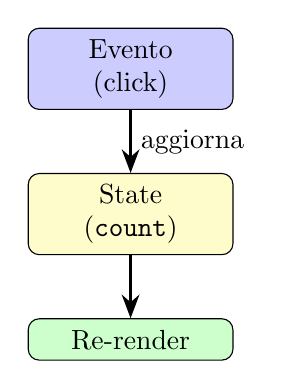
\begin{tikzpicture}[node distance=8mm,
					box/.style={draw, rectangle, rounded corners, minimum width=2.6cm, align=center, inner sep=4pt},
					arrow/.style={-{Stealth[length=3mm]}, thick}]
					\node[box, fill=yellow!20] (state) {State\\(\texttt{count})};
					\node[box, fill=blue!20, above=of state] (event) {Evento\\(click)};
					\node[box, fill=green!20, below=of state] (render) {Re-render};
					
					\draw[arrow] (event) -- (state) node[midway, right] {aggiorna};
					\draw[arrow] (state) -- (render);
				\end{tikzpicture}
			\end{column}
		\end{columns}
		
		\begin{alertblock}{Importante}
			Modificare lo \texttt{state} esclusivamente tramite \texttt{this.setState()} (o tramite
			la callback di setState quando il nuovo valore dipende dallo stato precedente). Non modificare
			direttamente \texttt{this.state}.
		\end{alertblock}
		
		\begin{block}{Nota}
			In componenti funzionali si usa l'hook \texttt{useState} per lo stesso scopo: \\
			\texttt{const [count, setCount] = useState(0);} e \texttt{setCount(c => c + 1)}.
		\end{block}
	\end{frame}
	
	
	% ========== SLIDE 15: STATE VS PROPS ==========
	\begin{frame}{State vs Props}
		\begin{center}
			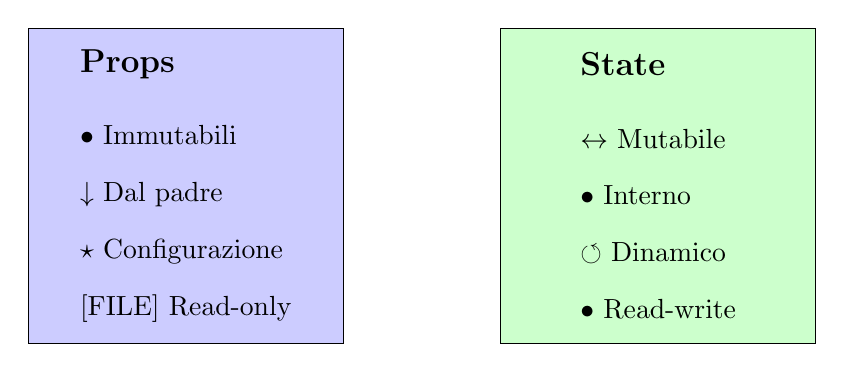
\begin{tikzpicture}
				% Props
				\node[draw, rectangle, fill=blue!20, minimum width=4cm, minimum height=4cm, align=left] at (-3,0) {
					\textbf{\large Props}\\[0.5cm]
					$\bullet$\ Immutabili\\[0.3cm]
					$\downarrow$\ Dal padre\\[0.3cm]
					$\star$\ Configurazione\\[0.3cm]
					[FILE]\ Read-only
				};
				
				% State
				\node[draw, rectangle, fill=green!20, minimum width=4cm, minimum height=4cm, align=left] at (3,0) {
					\textbf{\large State}\\[0.5cm]
					$\leftrightarrow$\ Mutabile\\[0.3cm]
					$\bullet$\ Interno\\[0.3cm]
					$\circlearrowleft$\ Dinamico\\[0.3cm]
					$\bullet$\ Read-write
				};
			\end{tikzpicture}
		\end{center}
		
		\begin{block}{Best Practice}
			\begin{itemize}
				\item Minimizzare i componenti con state
				\item Usare props per passare dati ai figli
				\item State solo dove necessario
			\end{itemize}
		\end{block}
	\end{frame}
	
	% ========== SLIDE 16: GERARCHIA COMPONENTI ==========
	\begin{frame}{Gerarchia di Componenti}
		\begin{center}
			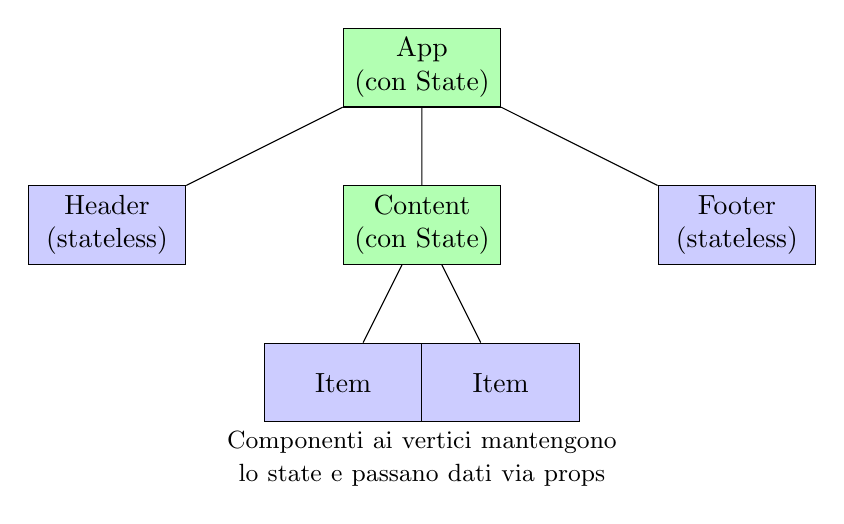
\begin{tikzpicture}[
				level 1/.style={sibling distance=4cm, level distance=2cm},
				level 2/.style={sibling distance=2cm, level distance=2cm},
				stateful/.style={rectangle, draw, fill=green!30, minimum width=2cm, minimum height=1cm, align=center},
				stateless/.style={rectangle, draw, fill=blue!20, minimum width=2cm, minimum height=1cm, align=center}
				]
				\node[stateful] {App\\(con State)}
				child {
					node[stateless] {Header\\(stateless)}
				}
				child {
					node[stateful] {Content\\(con State)}
					child {node[stateless] {Item}}
					child {node[stateless] {Item}}
				}
				child {
					node[stateless] {Footer\\(stateless)}
				};
				
				\node[below=4.5cm, text width=8cm, align=center] {
					\small Componenti ai vertici mantengono lo state e passano dati via props
				};
			\end{tikzpicture}
		\end{center}
	\end{frame}
	
	% ========== SLIDE 17: GESTIONE EVENTI ==========
	\begin{frame}[fragile]{Gestione degli Eventi}
		\begin{lstlisting}[language=JavaScript, basicstyle=\ttfamily\footnotesize]
			class Button extends React.Component {
				handleClick(e) {
					console.log('Pulsante premuto - Evento: ' + e.type);
				}
				
				render() {
					return (
					<button onClick={this.handleClick}>
					Cliccami
					</button>
					);
				}
			}
		\end{lstlisting}
		
		\begin{center}
			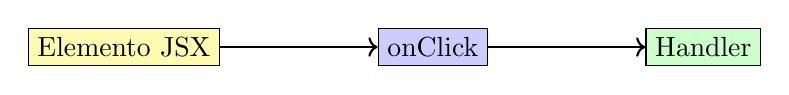
\begin{tikzpicture}[node distance=2cm]
				\node[draw, rectangle, fill=yellow!30] (element) {Elemento JSX};
				\node[draw, rectangle, fill=blue!20, right=of element] (event) {onClick};
				\node[draw, rectangle, fill=green!20, right=of event] (handler) {Handler};
				
				\draw[->, thick] (element) -- (event);
				\draw[->, thick] (event) -- (handler);
			\end{tikzpicture}
		\end{center}
		
		\begin{block}{Eventi comuni}
			onClick, onChange, onSubmit, onMouseOver, onKeyPress, ...
		\end{block}
	\end{frame}
	
	% ========== SLIDE 18: BINDING THIS ==========
	\begin{frame}[fragile]{Binding del this negli Eventi}
		\textbf{Problema}: accedere allo state nell'handler
		
		\vspace{0.3cm}
		
		\begin{columns}
			\column{0.5\textwidth}
			\textbf{Versione 1: Bind nel costruttore}
			\begin{lstlisting}[language=JavaScript, basicstyle=\ttfamily\tiny]
				constructor(props) {
					super(props);
					this.state = {on: false};
					this.handleClick = 
					this.handleClick.bind(this);
				}
				
				handleClick() {
					this.setState({
						on: !this.state.on
					});
				}
				
				render() {
					return (
					<button onClick=
					{this.handleClick}>
					</button>
					);
				}
			\end{lstlisting}
			
			\column{0.5\textwidth}
			\textbf{Versione 2: Arrow function}
			\begin{lstlisting}[language=JavaScript, basicstyle=\ttfamily\tiny]
				constructor(props) {
					super(props);
					this.state = {on: false};
					// NO bind necessario
				}
				
				handleClick() {
					this.setState({
						on: !this.state.on
					});
				}
				
				render() {
					return (
					<button onClick=
					{() => this.handleClick()}>
					</button>
					);
				}
			\end{lstlisting}
		\end{columns}
	\end{frame}
	
	% ========== SLIDE 19: ESEMPIO CALCOLATRICE INTRO ==========
	\begin{frame}{Esempio: Calcolatrice React}
		\begin{columns}
			\column{0.4\textwidth}
			\begin{center}
				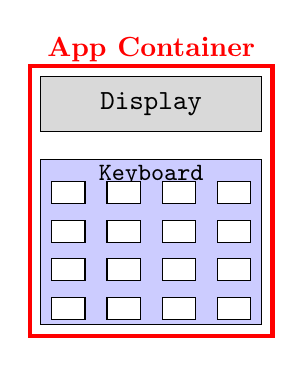
\begin{tikzpicture}[scale=0.7]
					% Display
					\draw[fill=gray!30] (0,3.5) rectangle (4,4.5);
					\node at (2,4) {\texttt{Display}};
					
					% Keyboard
					\draw[fill=blue!20] (0,0) rectangle (4,3);
					\node at (2,2.7) {\small\texttt{Keyboard}};
					
					% Buttons
					\foreach \x in {0.5,1.5,2.5,3.5} {
						\foreach \y in {0.3,1.0,1.7,2.4} {
							\draw[fill=white] (\x-0.3,\y-0.2) rectangle (\x+0.3,\y+0.2);
						}
					}
					
					% Container
					\draw[red, ultra thick] (-0.2,-0.2) rectangle (4.2,4.7);
					\node[red] at (2,5) {\textbf{App Container}};
				\end{tikzpicture}
			\end{center}
			
			\column{0.6\textwidth}
			\textbf{Componenti necessari:}
			\begin{enumerate}
				\item \textcolor{green!60!black}{Display} (figlio, stateless)
				\begin{itemize}
					\item Visualizza espressione
					\item Visualizza risultato
				\end{itemize}
				
				\item \textcolor{blue}{Keyboard} (figlio, stateless)
				\begin{itemize}
					\item Bottoni numerici
					\item Operatori aritmetici
				\end{itemize}
				
				\item \textcolor{red}{App} (padre, stateful)
				\begin{itemize}
					\item Gestisce lo state
					\item Gestisce eventi
					\item Compone i componenti
				\end{itemize}
			\end{enumerate}
		\end{columns}
	\end{frame}
	
	% ========== SLIDE 20: CALCOLATRICE DISPLAY ==========
	\begin{frame}[fragile]{Calcolatrice: Componente Display}
		\begin{lstlisting}[language=JavaScript, basicstyle=\ttfamily\footnotesize]
			function Display(props) {
				return (
				<div className="display">
				<input 
				type="text" 
				value={props.value} 
				readOnly 
				/>
				</div>
				);
			}
		\end{lstlisting}
		
		\begin{block}{Caratteristiche}
			\begin{itemize}
				\item Componente \textbf{function} (stateless)
				\item Riceve il valore da visualizzare tramite \textbf{props}
				\item Campo di input in sola lettura
				\item Riutilizzabile
			\end{itemize}
		\end{block}
	\end{frame}
	
	% ========== SLIDE 21: CALCOLATRICE KEYBOARD ==========
	\begin{frame}[fragile]{Calcolatrice: Componente Keyboard}
		\begin{lstlisting}[language=JavaScript, basicstyle=\ttfamily\tiny]
			function Keyboard(props) {
				return (
				<div className="keyboard">
				<button onClick={() => props.onButtonClick('7')}>7</button>
				<button onClick={() => props.onButtonClick('8')}>8</button>
				<button onClick={() => props.onButtonClick('9')}>9</button>
				<button onClick={() => props.onButtonClick('+')}>+</button>
				{/* altri bottoni... */}
				<button onClick={() => props.onButtonClick('=')}>=</button>
				</div>
				);
			}
		\end{lstlisting}
		
		\begin{block}{Caratteristiche}
			\begin{itemize}
				\item Riceve funzione handler tramite props
				\item Ogni bottone invoca \texttt{props.onButtonClick}
				\item Non gestisce logica, solo presentazione
			\end{itemize}
		\end{block}
	\end{frame}
	
	% ========== SLIDE 22: CALCOLATRICE APP ==========
	\begin{frame}[fragile]{Calcolatrice: Componente App}
		\begin{lstlisting}[language=JavaScript, basicstyle=\ttfamily\tiny]
			class App extends React.Component {
				constructor(props) {
					super(props);
					this.state = { expression: '', result: '' };
				}
				
				handleButtonClick = (value) => {
					if (value === '=') {
						try {
							this.setState({ result: eval(this.state.expression) });
						} catch (e) {
							this.setState({ result: 'Errore' });
						}
					} else if (value === 'C') {
						this.setState({ expression: '', result: '' });
					} else {
						this.setState({ expression: this.state.expression + value });
					}
				}
				
				render() {
					return (
					<div>
					<Display value={this.state.expression || this.state.result} />
					<Keyboard onButtonClick={this.handleButtonClick} />
					</div>
					);
				}
			}
		\end{lstlisting}
	\end{frame}
	
	% ========== SLIDE 23: FLUSSO DATI ==========
	\begin{frame}{Flusso dei Dati nella Calcolatrice}
		\begin{center}
			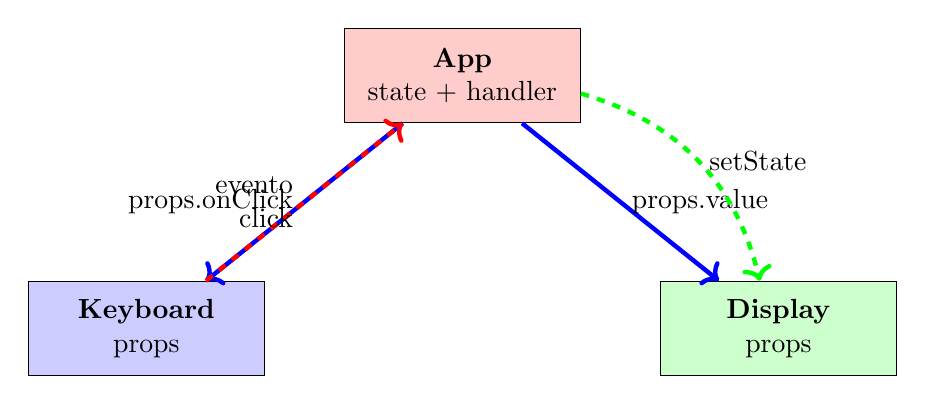
\begin{tikzpicture}[
				node distance=2cm,
				component/.style={rectangle, draw, minimum width=3cm, minimum height=1.2cm, align=center},
				arrow/.style={->, ultra thick}
				]
				% Componenti
				\node[component, fill=red!20] (app) {\textbf{App}\\state + handler};
				\node[component, fill=blue!20, below left=2cm and 1cm of app] (keyboard) {\textbf{Keyboard}\\props};
				\node[component, fill=green!20, below right=2cm and 1cm of app] (display) {\textbf{Display}\\props};
				
				% Frecce props down
				\draw[arrow, blue] (app) -- node[left, black] {props.onClick} (keyboard);
				\draw[arrow, blue] (app) -- node[right, black] {props.value} (display);
				
				% Freccia evento up
				\draw[arrow, red, dashed] (keyboard) -- node[left, black, align=right] {evento\\click} (app);
				
				% Update display
				\draw[arrow, green, dashed] (app) to[bend left=30] node[right, black] {setState} (display);
			\end{tikzpicture}
		\end{center}
		
		\begin{alertblock}{Pattern}
			\textbf{Top-down data flow}: i dati fluiscono dall'alto verso il basso tramite props
		\end{alertblock}
	\end{frame}
	
	% ========== SLIDE 24: MODULI E RIUSABILITA ==========
	\begin{frame}{Modularità e Riusabilità}
		\begin{block}{Problema}
			Applicazione monolitica in un singolo file = difficile riutilizzare componenti
		\end{block}
		
		\begin{center}
			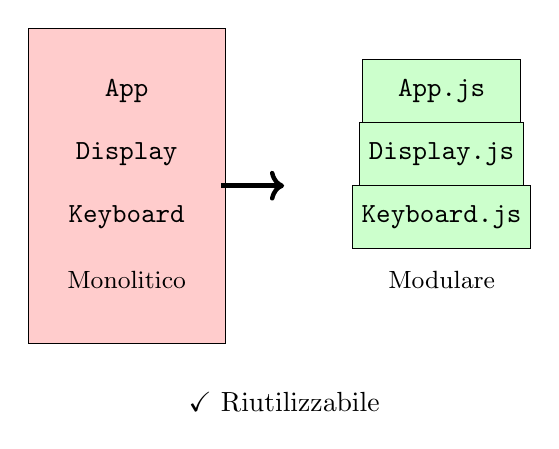
\begin{tikzpicture}[scale=0.8]
				% File monolitico
				\node[draw, rectangle, fill=red!20, minimum width=2.5cm, minimum height=4cm] at (-2,0) {};
				\node at (-2,1.5) {\texttt{App}};
				\node at (-2,0.5) {\texttt{Display}};
				\node at (-2,-0.5) {\texttt{Keyboard}};
				\node at (-2,-1.5) {\small Monolitico};
				
				\draw[->, ultra thick] (-0.5,0) -- (0.5,0);
				
				% File separati
				\node[draw, rectangle, fill=green!20, minimum width=2cm, minimum height=0.8cm] at (3,1.5) {\texttt{App.js}};
				\node[draw, rectangle, fill=green!20, minimum width=2cm, minimum height=0.8cm] at (3,0.5) {\texttt{Display.js}};
				\node[draw, rectangle, fill=green!20, minimum width=2cm, minimum height=0.8cm] at (3,-0.5) {\texttt{Keyboard.js}};
				\node at (3,-1.5) {\small Modulare};
				
				\node[below=2.5cm] at (0.5,0) {$\checkmark$\ Riutilizzabile};
			\end{tikzpicture}
		\end{center}
		
		\begin{block}{Soluzione}
			Creare file separati per ogni componente con import/export
		\end{block}
	\end{frame}
	
	% ========== SLIDE 25: IMPORT EXPORT ==========
	\begin{frame}[fragile]{Import ed Export}
		\textbf{Display.js:}
		\begin{lstlisting}[language=JavaScript, basicstyle=\ttfamily\footnotesize]
			import React from 'react';
			
			function Display(props) {
				return <div>{props.value}</div>;
			}
			
			export default Display;
		\end{lstlisting}
		
		\textbf{App.js:}
		\begin{lstlisting}[language=JavaScript, basicstyle=\ttfamily\footnotesize]
			import React from 'react';
			import Display from './Display';
			import Keyboard from './Keyboard';
			
			class App extends React.Component {
				// ...
			}
			
			export default App;
		\end{lstlisting}
	\end{frame}
	
	% ========== SLIDE 26: TOOLCHAIN ==========
	\begin{frame}{Toolchain di Sviluppo}
		\begin{block}{Cos'è una Toolchain?}
			Insieme di strumenti integrati che facilitano lo sviluppo professionale
		\end{block}
		
		\begin{center}
			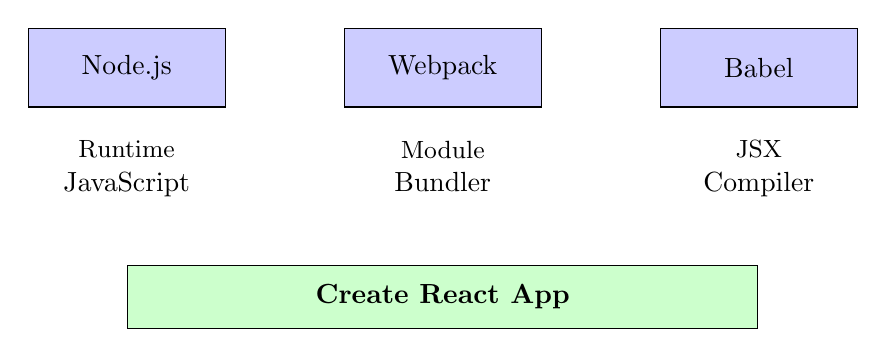
\begin{tikzpicture}[
				tool/.style={rectangle, draw, fill=blue!20, minimum width=2.5cm, minimum height=1cm},
				node distance=1.5cm
				]
				\node[tool] (nodejs) {Node.js};
				\node[tool, right=of nodejs] (webpack) {Webpack};
				\node[tool, right=of webpack] (babel) {Babel};
				
				\node[below=0.3cm of nodejs, align=center] {\small Runtime\\JavaScript};
				\node[below=0.3cm of webpack, align=center] {\small Module\\Bundler};
				\node[below=0.3cm of babel, align=center] {\small JSX\\Compiler};
				
				\node[draw, rectangle, fill=green!20, minimum width=8cm, minimum height=0.8cm, below=2cm of webpack] {
					\textbf{Create React App}
				};
			\end{tikzpicture}
		\end{center}
		
		\begin{block}{Vantaggi}
			\begin{itemize}
				\item Hot reload durante sviluppo
				\item Individuazione errori
				\item Ottimizzazione per produzione
				\item Configurazione zero
			\end{itemize}
		\end{block}
	\end{frame}
	
	% ========== SLIDE 27: COMANDI NPM ==========
	\begin{frame}[fragile]{Comandi NPM Principali}
		\begin{block}{npm start}
			\begin{lstlisting}[language=bash]
				npm start
			\end{lstlisting}
			Avvia server di sviluppo su \texttt{localhost:3000}\\
			Hot reload automatico delle modifiche
		\end{block}
		
		\begin{block}{npm run build}
			\begin{lstlisting}[language=bash]
				npm run build
			\end{lstlisting}
			Crea directory \texttt{build/} con file ottimizzati per produzione\\
			Pronta per deploy su web server
		\end{block}
		
		\begin{center}
			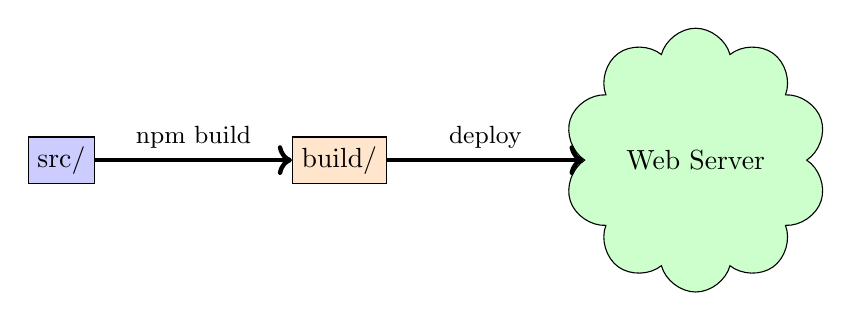
\begin{tikzpicture}[node distance=2.5cm]
				\node[draw, rectangle, fill=blue!20] (src) {src/};
				\node[draw, rectangle, fill=orange!20, right=of src] (build) {build/};
				\node[draw, cloud, fill=green!20, right=of build] (server) {Web Server};
				
				\draw[->, ultra thick] (src) -- node[above] {\small npm build} (build);
				\draw[->, ultra thick] (build) -- node[above] {\small deploy} (server);
			\end{tikzpicture}
		\end{center}
	\end{frame}
	
	% ========== SLIDE 28: BUNDLING ==========
	\begin{frame}{Application Bundling}
		\begin{center}
			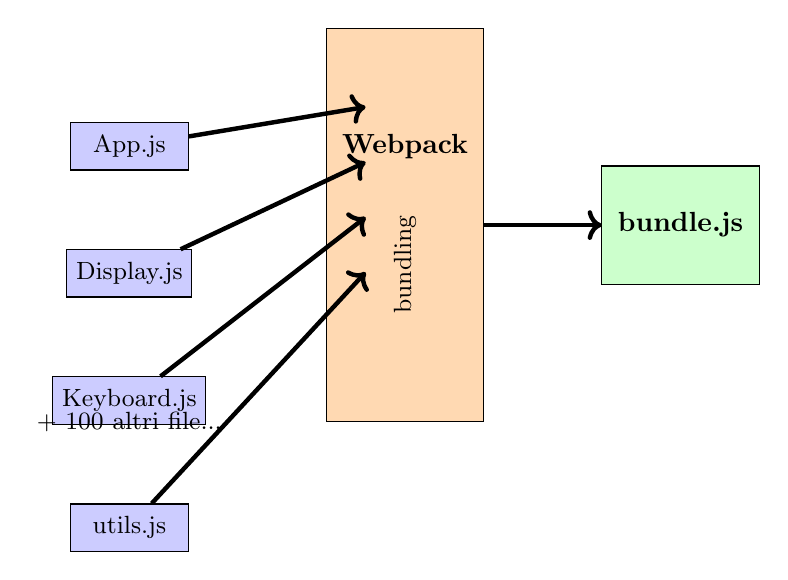
\begin{tikzpicture}[
				file/.style={rectangle, draw, fill=blue!20, minimum width=1.5cm, minimum height=0.6cm},
				node distance=1cm
				]
				% File sorgenti
				\node[file] (app) {\small App.js};
				\node[file, below=of app] (display) {\small Display.js};
				\node[file, below=of display] (keyboard) {\small Keyboard.js};
				\node[file, below=of keyboard] (utils) {\small utils.js};
				\node at (0,-3.5) {\small + 100 altri file...};
				
				% Webpack
				\node[draw, rectangle, fill=orange!30, minimum width=2cm, minimum height=5cm] at (3.5,-1) {};
				\node at (3.5,0) {\textbf{Webpack}};
				\node[rotate=90] at (3.5,-1.5) {\small bundling};
				
				% Bundle output
				\node[draw, rectangle, fill=green!20, minimum width=2cm, minimum height=1.5cm] at (7,-1) {
					\textbf{bundle.js}
				};
				
				\draw[->, ultra thick] (app) -- (3,0.5);
				\draw[->, ultra thick] (display) -- (3,-0.2);
				\draw[->, ultra thick] (keyboard) -- (3,-0.9);
				\draw[->, ultra thick] (utils) -- (3,-1.6);
				
				\draw[->, ultra thick] (4.5,-1) -- (6,-1);
			\end{tikzpicture}
		\end{center}
		
		\begin{block}{Webpack}
			Tool che combina tutti i moduli JavaScript in un unico file ottimizzato
		\end{block}
	\end{frame}
	
	% ========== SLIDE 29: ESERCIZI ==========
	\begin{frame}{Esercizi Proposti}
		\begin{block}{Esercizio 1: Doppio Display}
			Modificare la calcolatrice per avere:
			\begin{itemize}
				\item Display 1: mostra l'espressione in composizione
				\item Display 2: mostra il risultato finale
				\item Tasto 'C': resetta entrambi i display
			\end{itemize}
			\textbf{Suggerimento}: riutilizzare il componente Display esistente!
		\end{block}
		
		\begin{block}{Esercizio 2: Calcolatrice Scientifica}
			Aggiungere funzionalità scientifiche:
			\begin{itemize}
				\item Nuovo tastierino con: $\log_e(x)$, $\sqrt{x}$, $e^x$, $\frac{1}{x}$
				\item Applicare operatori all'espressione corrente
				\item Posizionare sotto la tastiera esistente
			\end{itemize}
		\end{block}
	\end{frame}
	
	% ========== SLIDE 30: BEST PRACTICES ==========
	\begin{frame}{Best Practices React}
		\begin{columns}
			\column{0.5\textwidth}
			\textbf{Struttura:}
			\begin{itemize}
				\item $\checkmark$\ Componenti piccoli e focalizzati
				\item $\checkmark$\ Separare logica e presentazione
				\item $\checkmark$\ Un componente per file
				\item $\checkmark$\ Naming chiaro e consistente
			\end{itemize}
			
			\vspace{0.5cm}
			
			\textbf{State Management:}
			\begin{itemize}
				\item $\checkmark$\ Minimizzare componenti stateful
				\item $\checkmark$\ State il più in alto possibile
				\item $\checkmark$\ Props per passare dati in basso
			\end{itemize}
			
			\column{0.5\textwidth}
			\textbf{Performance:}
			\begin{itemize}
				\item $\checkmark$\ Evitare binding in render
				\item $\checkmark$\ Usare keys nelle liste
				\item $\checkmark$\ Componenti puri quando possibile
			\end{itemize}
			
			\vspace{0.5cm}
			
			\textbf{Codice:}
			\begin{itemize}
				\item $\checkmark$\ JSX leggibile e indentato
				\item $\checkmark$\ Commenti dove necessario
				\item $\checkmark$\ PropTypes per validazione
				\item $\checkmark$\ Testing dei componenti
			\end{itemize}
		\end{columns}
	\end{frame}
	Fraticelli
	% ========== SLIDE 31: RISORSE ==========
	\begin{frame}{Risorse Utili}
		\begin{block}{Documentazione Ufficiale}
			\begin{itemize}
				\item \textbf{React}: \url{https://reactjs.org/docs}
				\item \textbf{Create React App}: \url{https://create-react-app.dev/}
				\item \textbf{Babel}: \url{https://babeljs.io/}
			\end{itemize}
		\end{block}
		
		\begin{block}{Tutorial e Guide}
			\begin{itemize}
				\item React Tutorial ufficiale
				\item FreeCodeCamp React Course
				\item React Patterns
				\item Awesome React (GitHub)
			\end{itemize}
		\end{block}
		
		\begin{block}{Tools}
			\begin{itemize}
				\item React Developer Tools (Chrome/Firefox)
				\item VS Code + ES7 React snippets
				\item CodeSandbox per prototipazione rapida
			\end{itemize}
		\end{block}
	\end{frame}
	
	% ========== SLIDE 32: CONCLUSIONI ==========
	\begin{frame}{Conclusioni}
		\begin{center}
			
\begin{tikzpicture}[scale=0.6]
				% React logo
				\draw[reactblue, ultra thick] (0,0) circle (2);
				\fill[reactblue] (0,0) circle (0.4);
				\draw[reactblue, ultra thick, rotate=60] (0,0) ellipse (4 and 1);
				\draw[reactblue, ultra thick, rotate=-60] (0,0) ellipse (4 and 1);
			\end{tikzpicture}
		\end{center}
		
		\begin{block}{Cosa abbiamo imparato}
			\begin{itemize}
				\item Fondamenti di React.js e Single Page Applications
				\item Componenti function e class
				\item Props e State
				\item Gestione eventi
				\item Sviluppo modulare con toolchain
				\item Pattern di composizione
			\end{itemize}
		\end{block}
		
		\begin{center}
			\Large\textbf{Buon lavoro con React!}
		\end{center}
	\end{frame}
	
	% ========== SLIDE 33: CONTATTI ==========
	\begin{frame}{Riferimenti}
		\begin{center}
			\Large\textbf{Tecnologie Web T}\\
			\large A.A. 2020--2021
			
			\vspace{1cm}
			
			\normalsize
			Home Page del corso:\\
			\url{http://lia.disi.unibo.it/Courses/twt2021-info/}
			
			\vspace{0.5cm}
			
			Versione elettronica:\\
			\texttt{L.06.React.pdf}\\
			\texttt{L.06.React-2p.pdf}
			
			\vspace{1cm}
			
			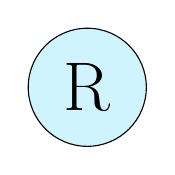
\begin{tikzpicture}
				\node[draw, circle, fill=reactblue!30, minimum size=1.5cm] {\Huge R};
			\end{tikzpicture}
		\end{center}
	\end{frame}
	
		
		\begin{frame}
			\titlepage
		\end{frame}
		
		\begin{frame}{Indice}
			\tableofcontents
		\end{frame}
		
		\section{Introduzione a React}
		
		\begin{frame}{Cos'è React?}
			\begin{columns}
				\column{0.6\textwidth}
				\begin{itemize}
					\item \textbf{Libreria JavaScript} creata da Facebook (Meta) nel 2013
					\item Per costruire \textbf{interfacce utente} interattive
					\item Basata su \textbf{componenti riutilizzabili}
					\item Approccio \textbf{dichiarativo}
					\item Utilizzata da: Facebook, Instagram, Netflix, Airbnb
				\end{itemize}
				
				\column{0.35\textwidth}
				\begin{center}
					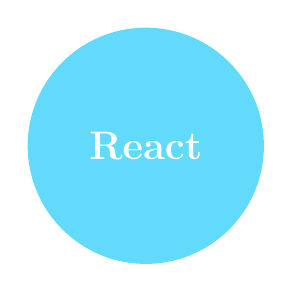
\begin{tikzpicture}
						\node[circle, fill=reactblue, minimum size=3cm] (react) {};
						\node[white, font=\Large\bfseries] at (react) {React};
					\end{tikzpicture}
				\end{center}
			\end{columns}
		\end{frame}
		
		\begin{frame}{Perché React?}
			\begin{block}{Vantaggi}
				\begin{itemize}
					\item [+] \textbf{Componenti riutilizzabili}: scrivi una volta, usa ovunque
					\item [+] \textbf{Virtual DOM}: aggiornamenti efficienti
					\item [+] \textbf{Flusso dati unidirezionale}: più facile da debuggare
					\item [+] \textbf{Ecosistema ricco}: migliaia di librerie
					\item [+] \textbf{Community enorme}: supporto e risorse abbondanti
				\end{itemize}
			\end{block}
		\end{frame}
		
		\section{Concetti Fondamentali}
		
		\begin{frame}[fragile]{Componenti}
			\begin{block}{Definizione}
				I componenti sono funzioni che restituiscono JSX
			\end{block}
			
			\begin{lstlisting}
				// Componente semplice
				function Benvenuto() @\{@
				return <h1>Ciao, benvenuto in React!</h1>;
				@\}@
				
				// Componente con props
				function Saluto(@\{@ nome @\}@) @\{@
				return <h1>Ciao, @\{@nome@\}@!</h1>;
				@\}@
			\end{lstlisting}
		\end{frame}
		
		\begin{frame}[fragile]{Props - Proprietà}
			\begin{block}{Definizione}
				Le \textbf{props} sono dati passati dal padre al figlio. Sono \textbf{immutabili}.
			\end{block}
			
			\begin{lstlisting}
				function TaskItem(@\{@ task, onDelete @\}@) @\{@
				return (
				<div>
				<span>@\{@task.text@\}@</span>
				<button onClick=@\{@() => onDelete(task.id)@\}@>
				Elimina
				</button>
				</div>
				);
				@\}@
			\end{lstlisting}
		\end{frame}
		
		\begin{frame}[fragile]{State - Lo Stato}
			\begin{block}{Definizione}
				Lo \textbf{state} contiene dati che cambiano e causano il ri-rendering.
			\end{block}
			
			\begin{lstlisting}
				import @\{@ useState @\}@ from 'react';
				
				function Contatore() @\{@
				const [conteggio, setConteggio] = useState(0);
				
				return (
				<div>
				<p>Hai cliccato @\{@conteggio@\}@ volte</p>
				<button onClick=@\{@() => setConteggio(conteggio + 1)@\}@>
				Incrementa
				</button>
				</div>
				);
				@\}@
			\end{lstlisting}
		\end{frame}
		
		\begin{frame}{State vs Props}
			\begin{center}
				\begin{tabular}{|l|p{5cm}|p{5cm}|}
					\hline
					\rowcolor{reactblue!30}
					\textbf{Caratteristica} & \textbf{Props} & \textbf{State} \\
					\hline
					Mutabilit\`a & Immutabili & Mutabili \\
					\hline
					Origine & Passate dal padre & Gestite dal componente \\
					\hline
					Modifica & NO & SI (con setState) \\
					\hline
					Re-render & NO & SI (quando cambia) \\
					\hline
				\end{tabular}
			\end{center}
			
			\vspace{0.5cm}
			\begin{alertblock}{Regola d'oro}
				Se un dato \textbf{cambia} $\rightarrow$ \texttt{useState}\\
				Se un dato e \textbf{passato dal padre} $\rightarrow$ props
			\end{alertblock}
		\end{frame}
		
		\section{Hooks Principali}
		
		\begin{frame}[fragile]{useState Hook}
			\begin{block}{Sintassi}
				\texttt{const [stato, setStato] = useState(valoreIniziale);}
			\end{block}
			
			\begin{lstlisting}
				function FormEsempio() @\{@
				const [nome, setNome] = useState('');
				const [eta, setEta] = useState(0);
				
				return (
				<input 
				value=@\{@nome@\}@
				onChange=@\{@(e) => setNome(e.target.value)@\}@
				/>
				);
				@\}@
			\end{lstlisting}
		\end{frame}
		
		\begin{frame}[fragile]{useEffect Hook}
			\begin{block}{Scopo}
				Eseguire \textbf{effetti collaterali}: chiamate API, sottoscrizioni, timer
			\end{block}
			
			\begin{lstlisting}
				import @\{@ useState, useEffect @\}@ from 'react';
				
				function Esempio() @\{@
				const [count, setCount] = useState(0);
				
				// Si esegue dopo ogni render
				useEffect(() => @\{@
				document.title = `Cliccato $@\{@count@\}@ volte`;
				@\}@);
				
				// Si esegue solo al mount
				useEffect(() => @\{@
				console.log('Componente montato!');
				@\}@, []);
				@\}@
			\end{lstlisting}
		\end{frame}
		
		\section{Applicazione Pratica}
		
		\begin{frame}[fragile]{Task Manager - Esempio Completo}
			\begin{lstlisting}[basicstyle=\ttfamily\footnotesize\color{white}]
				function App() @\{@
				const [tasks, setTasks] = useState([]);
				const [inputValue, setInputValue] = useState('');
				
				const addTask = () => @\{@
				if (inputValue.trim() === '') return;
				setTasks([...tasks, @\{@
				id: Date.now(),
				text: inputValue,
				completed: false
				@\}@]);
				setInputValue('');
				@\}@;
				
				const deleteTask = (id) => @\{@
				setTasks(tasks.filter(task => task.id !== id));
				@\}@;
				@\}@
			\end{lstlisting}
		\end{frame}
		
		\begin{frame}[fragile]{Immutabilit\`a dello State}
			\begin{alertblock}{Regola Importante}
				\textbf{NON} modificare mai direttamente lo state!
			\end{alertblock}
			
			\begin{columns}
				\column{0.48\textwidth}
				\textbf{\textcolor{red}{SBAGLIATO}}
				\begin{lstlisting}[numbers=none]
					// NON fare cosi!
					tasks.push(newTask);
					setTasks(tasks);
				\end{lstlisting}
				
				\column{0.48\textwidth}
				\textbf{\textcolor{green}{CORRETTO}}
				\begin{lstlisting}[numbers=none]
					// Crea nuovo array
					setTasks([
					...tasks, 
					newTask
					]);
				\end{lstlisting}
			\end{columns}
		\end{frame}
		
		\begin{frame}{Best Practices}
			\begin{enumerate}
				\item \textbf{Un componente, una responsabilit\`a}
				\begin{itemize}
					\item Mantieni i componenti piccoli e focalizzati
				\end{itemize}
				
				\item \textbf{Denomina chiaramente}
				\begin{itemize}
					\item Componenti: PascalCase (\texttt{TaskItem})
					\item Props/variabili: camelCase (\texttt{onDelete})
				\end{itemize}
				
				\item \textbf{Immutabilit\`a dello state}
				\begin{itemize}
					\item Non modificare mai direttamente lo state
				\end{itemize}
				
				\item \textbf{Key univoche nelle liste}
				\begin{itemize}
					\item Mai usare l'indice come key
				\end{itemize}
			\end{enumerate}
		\end{frame}
		
		\begin{frame}{Errori Comuni da Evitare}
			\begin{alertblock}{1. Modificare direttamente lo state}
				Non fare: \texttt{tasks[0] = newTask;}
			\end{alertblock}
			
			\begin{alertblock}{2. Chiamare hooks condizionalmente}
				Gli hook vanno sempre in cima alla funzione
			\end{alertblock}
			
			\begin{alertblock}{3. Dimenticare le dipendenze in useEffect}
				Porta a bug difficili da trovare
			\end{alertblock}
			
			\begin{alertblock}{4. Usare l'indice come key}
				Usa ID univoci invece di indici
			\end{alertblock}
		\end{frame}
		
		\section{Prossimi Passi}
		
		\begin{frame}{Argomenti Avanzati}
			\begin{columns}
				\column{0.5\textwidth}
				\textbf{Hooks Avanzati:}
				\begin{itemize}
					\item useContext
					\item useReducer
					\item useMemo
					\item useCallback
					\item useRef
				\end{itemize}
				
				\column{0.5\textwidth}
				\textbf{Concetti:}
				\begin{itemize}
					\item React Router
					\item Form avanzati
					\item Chiamate API
					\item State Management
					\item Testing
				\end{itemize}
			\end{columns}
		\end{frame}
		
		\begin{frame}{Risorse per Imparare}
			\begin{block}{Documentazione Ufficiale}
				\url{https://react.dev/} - Tutorial interattivi
			\end{block}
			
			\begin{block}{Pratica}
				\begin{itemize}
					\item Crea progetti reali (TODO app, blog)
					\item Contribuisci a progetti open source
					\item Partecipa a coding challenges
				\end{itemize}
			\end{block}
		\end{frame}
		
		\begin{frame}{Riepilogo}
			\begin{center}
				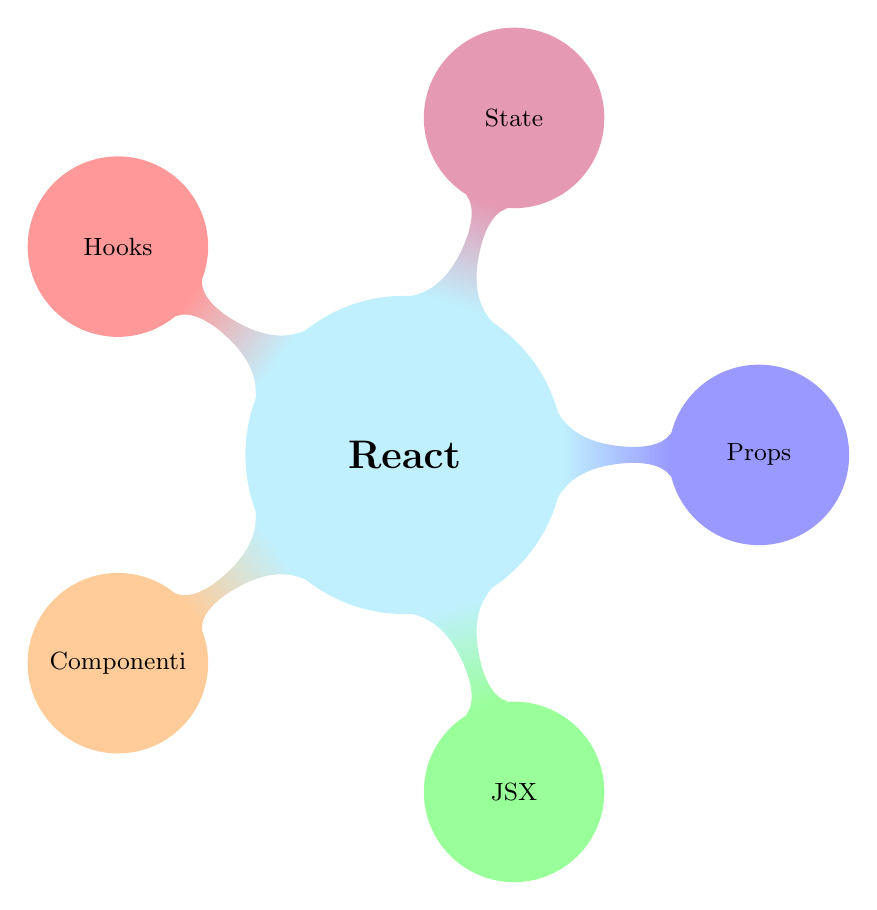
\begin{tikzpicture}[mindmap, grow cyclic, every node/.style=concept, concept color=reactblue!40,
					level 1/.append style={level distance=4.5cm,sibling angle=72}]
					
					\node[concept, font=\Large\bfseries] {React}
					child [concept color=orange!40] { node {Componenti} }
					child [concept color=green!40] { node {JSX} }
					child [concept color=blue!40] { node {Props} }
					child [concept color=purple!40] { node {State} }
					child [concept color=red!40] { node {Hooks} };
				\end{tikzpicture}
			\end{center}
		\end{frame}
		
		\begin{frame}
			\Huge Domande?
			\vspace{1cm}
			
			\normalsize
			Email: fedeli.massimo@iisfermisacconiceciap.edu.it\\
			GitHub: github.com/massimof79
			
			\vspace{1cm}
			\Large Grazie per l'attenzione!
		\end{frame}
		
	\end{document}
